\documentclass{UoNMCHA}
\usepackage[authoryear]{natbib}
\usepackage{array,booktabs} % For nice tables
\usepackage{amsmath,amsfonts,amssymb} % For nice maths
\usepackage{color}
\usepackage{enumerate}
\usepackage{listings}
\usepackage{subfig}
\usepackage{hyperref}
\usepackage{float}
\usepackage[parfill]{parskip}   % For replacing paragraph indenting with a newline instead
\usepackage{pdfpages}
\usepackage[australian]{babel} % This line sets the language to Australian English



% Number equations per section
\numberwithin{equation}{section}

\hypersetup{
%    bookmarks=true,         % show bookmarks bar?
%    unicode=false,          % non-Latin characters in AcrobatÕs bookmarks
%    pdftoolbar=true,        % show AcrobatÕs toolbar?
%    pdfmenubar=true,        % show AcrobatÕs menu?
%    pdffitwindow=false,     % window fit to page when opened
%    pdfstartview={FitH},    % fits the width of the page to the window
%    pdftitle={My title},    % title
%    pdfauthor={Author},     % author
%    pdfsubject={Subject},   % subject of the document
%    pdfcreator={Creator},   % creator of the document
%    pdfproducer={Producer}, % producer of the document
%    pdfkeywords={keyword1} {key2} {key3}, % list of keywords
%    pdfnewwindow=true,      % links in new window
    colorlinks=true,       % false: boxed links; true: colored links
    linkcolor=blue,          % color of internal links
    citecolor=blue,        % color of links to bibliography
%    filecolor=magenta,      % color of file links
    urlcolor=blue           % color of external links
}

\definecolor{MATLABKeyword}{rgb}{0,0,1}
\definecolor{MATLABComment}{rgb}{0.1328125,0.54296875,0.1328125}
\definecolor{MATLABString}{rgb}{0.625,0.125,0.9375}

\lstset{language=Matlab,
    basicstyle=\small\ttfamily,
    keywordstyle=\color{MATLABKeyword},
    %identifierstyle=,
    commentstyle=\color{MATLABComment},
    stringstyle=\color{MATLABString},
    numberstyle=\tiny,
    %numbers=left,
    basewidth=0.5em}



\firstpage{1}    % Set page number for first page
\UoNMCHAreportNo{MECH4841 Part A [B]} %Report number
\UoNMCHAyear{2013}   % Year
\shorttitle{FYP Report - Short Title} %For odd pages
%%%%%%%%%%%%%%%%%%%%%%%%%%%%%%%%%%%%%%%%%%%%%%%%%%%%
% Include the PDF title page


\begin{document}
\title{Autonomous Object Evasion, and Interception Using the Quanser QDrone\\ \ \\
{\small Final Year Project Report - ENGG4801A \\May 2024}}
\author[UoNMCHA]{Evan Byrne}
\address[UoNMCHA]{
Student of Mechatronics Engineering,\\
The University of Newcastle, Callaghan, NSW 2308, AUSTRALIA \\
Student Number: 3349681 \\
E-mail: \href{mailto:Evan.Byrne@uon.edu.au}{\textsf{Evan.Byrne@uon.edu.au}}}
%%%%%%%%%%%%%%%%%%%%%%%%%%%%%%%%%%%
\maketitle
\onecolumn

\vspace{-5mm}
\section*{Abstract}
\vspace{5mm}
This report focuses on a project in which the Quanser QDrone \cite{website:Quanser} is required to detect an object, specifically a ball in this scenario, and autonomously recognize and manoeuvre to either avoid or intercept it. This project explores various control systems and advanced object detection capabilities of current unmanned aerial vehicles (UAVs), aiming to enhance trajectory estimation for practical applications such as automated package retrieval and delivery. 
The current methodology for addressing this challenge involves the use of a Vicon System \cite{website:Vicon}. However, the project's ultimate goal is to achieve complete autonomy by relying solely on onboard sensors, cameras, and computational resources. Currently, MATLAB simulations show that nonlinear model predictive control (NMPC) \cite{website:NLMPC} is able to effectively capture the states of the QDrone. When coupling this with the ball trajectory, simulations show the QDrone successfully intercepting the object.

\newpage
\tableofcontents
\newpage

\section{Introduction}
The utilization of UAVs has significantly expanded across various sectors, driven by enhancements in their design and control systems. This project specifically addresses the autonomous capabilities of the Quanser QDrone for object detection and interaction tasks, which are critical in fields such as automated delivery and emergency response. The challenge lies in enabling the QDrone to identify and respond to dynamic objects, such as a moving ball, using only its onboard computational tools, rather than relying solely on external systems like the Vicon System.

Initially, this project leverages said Vicon System to provide accurate spatial tracking and support the development and testing of control algorithms. The project explores the adaptation and integration of advanced control systems and object detection technologies that have been traditionally used in less dynamic settings. Employing nonlinear model predictive control (NMPC) and Kalman Filter algorithms, the project aims to enhance the drone's ability to make real-time decisions based on the trajectory data of moving objects. The ultimate goal is to develop a fully autonomous UAV system capable of performing complex manoeuvres without human intervention, thereby pushing the boundaries of what autonomous drones can achieve in practical applications. 

This endeavour not only aims to advance the technological capabilities of UAVs but also to provide scalable solutions that could transform industries by enabling more sophisticated autonomous operations.



\section{Literature Review}


\subsection{System Dynamics}

\subsubsection{Quadrotor Dynamics}
All mathematical models for quadrotor UAVs depend on the blade orientation, which can be either a plus (+) configuration or a cross (X) configuration as seen in Figure.\ref{fig:QuadrotorConfigandRef}. The plus configuration aligns each rotor with the primary axes, resulting in symmetrical thrust distribution along these axes. This alignment allows for easier prediction and simplified control algorithms, making it an advantageous choice for straightforward control implementations and basic flight stability. This simplicity also introduces drawbacks, such as reduced manoeuvrability as well as increased complexity in sensor and camera placement. Alternatively, the X configuration allows for easier sensor placement and better stability, manoeuvrability, and aerodynamic efficiency; however, these benefits come at the cost of more complex control algorithms \cite{article:CrossVsPlus}.  

\begin{figure}[H]
    \centering
    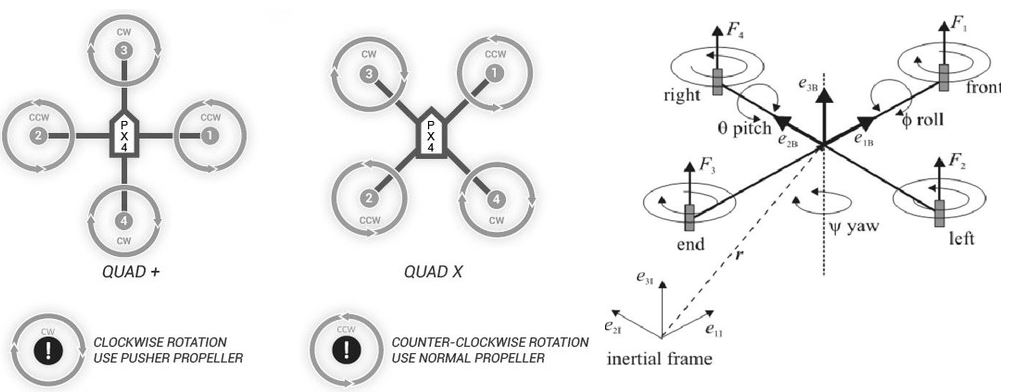
\includegraphics[width=\linewidth]{Figures/QuadrotorRefFrameandConfig.JPG}
    \caption{Quadrotor Configuration and Reference Frames}
    \label{fig:QuadrotorConfigandRef} % Add label for referencing
\end{figure}

Once a quadrotor orientation is established, the system dynamics can be derived. Quadrotors are six-degree-of-freedom (DOF) systems, encompassing three rotational and three translational movements. These movements are controlled using four individual thrust inputs, each dependent on the motor and blade on each arm. For the majority of literature, such as {\cite{website:Quadrotorsystemmodeling}}, the torques and forces created from each thrust about the primary axes form the basis of the model. Although this is a common approach in modelling quadrotors, due to the complexity of the system, models can vary from quite low-fidelity models to extremely high-fidelity models that encompass additional forces such as gyroscopic and drag forces. These varying levels of model fidelity allow researchers and engineers to balance the need for accuracy with computational efficiency, depending on the specific application and result in the lower fidelity models being more prevalent.

Regardless of the model's fidelity, an accurate representation of quadrotor dynamics necessitates the proper application of reference frames and the implementation of Euler-Newton and Euler-Lagrange equations \cite{IntroductionToRobotics}. Reference frames such as the ones shown in Figure \ref{fig:QuadrotorConfigandRef} are crucial for understanding the motion relative to different points of view, whether fixed or moving. The Euler-Newton method applies forces and torques to derive the equations of motion, while the Euler-Lagrange approach offers a generalised formulation ideal for capturing complex dynamics. These theoretical foundations are essential for developing robust models that can accurately predict and control the UAV's behaviour under various conditions 

As previously mentioned, quadrotors are nonlinear systems which inherently result in nonlinear models. Due to this, many control algorithms require the system to be linearised. This linearisation involves approximating the nonlinear dynamics around a specific operating point by taking the Jacobian {\cite{website:LinearisationandJacobian}}, thereby making it possible to apply linear control techniques. 

\subsubsection{Object Dynamics}
The kinematics and dynamics of objects travelling through the air can range from simplistic to complex, depending on the geometry of the object and the fidelity of the chosen model. Idealised projectile motion problems allow for easy estimation of trajectory, time of flight, and position by neglecting all external forces except gravity {\cite{website:ProjectilMotion}}. This approach simplifies analysis but overlooks critical factors that affect real-world objects.

As the complexity of the object increases, understanding the forces acting on it becomes significantly harder. Factors such as mass, surface area, and surface finish play major roles in determining drag forces, rotational biases, and asymmetrical rotation. Aerodynamic effects, such as the Magnus effect, and surface roughness can impact drag and lift characteristics. Computational fluid dynamics (CFD) simulations and wind tunnel experiments are often used to study these effects in detail. While idealised models offer simplicity, real-world dynamics require consideration of various physical phenomena to achieve accurate predictions.


\subsection{Controllers}
Refining and developing control strategies is vital for enabling quadrotors to perform complex tasks such as catching a ball. These strategies are designed to enhance the agility, stability, and precision of quadrotor systems, which are inherently unstable and require constant adjustments to maintain flight. From the straightforward control strategies such as Proportional-Derivative (PD) control to the more sophisticated Proportional-Integral-Derivative (PID) control, and extending further to advanced techniques like Linear Quadratic Regulator (LQR) control, Model Predictive Control (MPC), and Nonlinear Model Predictive Control (NMPC), researchers have developed and refined various methods to address the challenges of quadrotor dynamics. Each of these control strategies offers distinct advantages and complexities, making them suitable for different aspects of quadrotor flight and task execution \cite{ControllersCompare}.

\subsubsection{PD Control}
Proportional-Derivative (PD) control is one of the simplest and most widely used control strategies in quadrotor systems due to its ease of implementation and effectiveness in improving transient response \cite{website:TransientResponse}. The PD controller adjusts the control input based on the current error and its rate of change, providing a balance between the speed of response and damping.

In discrete time, the PD control law can be expressed as:
\begin{equation}
u[k] = K_p e[k] + K_d \frac{e[k] - e[k-1]}{T_s}
\end{equation}
where \( u[k] \) is the control input at the \( k \)-th sample, \( e[k] \) is the error at the \( k \)-th sample, and \( T_s \) is the sampling period \cite{PID}.

In the context of quadrotor control, the error \( e(t) \) or \( e[k] \) can be the difference between the desired and actual positions or angles. By tuning \( K_p \) and \( K_d \), the PD controller can achieve a fast and stable response, minimizing overshoot and settling time.
\subsubsection{PID Control}
Proportional-Integral-Derivative (PID) control builds upon the principles of PD control by adding an integral term to address the accumulation of past errors, which can help eliminate steady-state errors . The inclusion of the integral action allows the controller to adjust the control input not only based on the current error and its rate of change but also on the cumulative sum of past errors \cite{PID}.

In discrete time, the PID control law can be expressed as:
\begin{equation}
u[k] = K_p e[k] + K_d \frac{e[k] - e[k-1]}{T_s} + K_i T_s \sum_{j=0}^{k} e[j]
\end{equation}
where \( u[k] \) is the control input at the \( k \)-th sample, \( e[k] \) is the error at the \( k \)-th sample, and \( T_s \) is the sampling period \cite{PID}.

Although the integral term excels at removing steady state error that the proportional and derivative terms alone cannot, it must be carefully tuned as excessive integral gain can lead to integral windup, causing large overshoot and potentially destabilizing the system \cite{website:intWindup}.

By combining the proportional, integral, and derivative actions, the PID controller can provide a balanced approach to managing both transient and steady-state performance. This makes it a versatile and widely used control strategy in various applications, including quadrotor control.

\subsubsection{Cost Function in Optimal Control}

When moving to more advanced control methods, cost functions are the mathematical tool used to assess the performance of a control system. A cost function provides a measure of how well the system is achieving its desired objectives, typically by penalizing deviations from a target state and the effort required to control the system. The goal of the control strategy is to minimize this cost function, thereby optimizing the system's performance \cite{costFunctions}.

A common form of cost function used in optimal control strategies is a quadratic function, which can be expressed as:
\begin{equation}
\label{quadraticCostEq}
J = \int_{0}^{\infty} \left( x(t)^T Q x(t) + u(t)^T R u(t) \right) dt,
\end{equation}
where:
\begin{itemize}
    \item \( x(t) \) represents the state deviations.
    \item \( u(t) \) represents the control efforts.
    \item \( Q \) and \( R \) are weighting matrices that determine the relative importance of state deviations and control efforts.
\end{itemize}

The cost function helps to ensure that the system states remain close to the desired values while using control inputs efficiently. By carefully choosing the weights \( Q \) and \( R \), the control strategy can balance precision and efficiency, making it effective for systems requiring optimal performance, such as quadrotor control \cite{website:QuadraticCost}.





\subsubsection{LQR Control}


Linear Quadratic Regulator (LQR) control is a fundamental optimal control strategy designed for linear systems. It aims to find the optimal set of control inputs that minimize a predefined cost function, balancing the trade-off between state deviations and control efforts. This makes LQR particularly effective for systems where precision and efficiency are crucial.

The LQR control strategy leverages the quadratic cost function as shown in (\ref{quadraticCostEq}) to determine the optimal feedback control law. By minimizing this cost function, LQR ensures that the system's state remains close to the desired trajectory while using control inputs efficiently. 


LQR is advantageous for quadrotor control due to its optimal control solution, robustness to disturbances, and guaranteed stability if the system is controllable. Its simplicity and computational efficiency make it suitable for real-time applications. However, LQR assumes linear system dynamics, which can be inaccurate for the highly nonlinear behaviour of quadrotors, particularly during aggressive manoeuvres. This reliance on accurate models and fixed gains can limit its adaptability to changing conditions. As a result, more advanced nonlinear control methods are often preferred for handling complex scenarios. \cite{website:LQR}


\subsubsection{MPC Control}

Model Predictive Control (MPC) is an advanced control strategy that optimizes control inputs by predicting future system behaviour over a finite time horizon, making it suitable for complex systems like quadrotors. MPC minimizes a cost function, typically in the form:

\begin{equation}
J = \sum_{k=0}^{N-1} \left( x[k]^T Q x[k] + u[k]^T R u[k] \right) + x[N]^T P x[N],
\end{equation}

where \( N \) is the prediction horizon, \( x[k] \) is the state vector, \( u[k] \) is the control input, and \( Q \), \( R \), and \( P \) are weighting matrices. The term \( x[N] \) represents the state of the system at the end of the prediction horizon, guiding the quadrotor towards achieving its target objectives \cite{MPC}.

MPC effectively manages state and input constraints, handles multivariable control problems, and anticipates future disturbances. However, it requires significant computational resources, relies on an accurate system model, and involves complex parameter tuning. Despite these challenges, MPC's predictive and optimization capabilities make it ideal for precision and adaptability in quadrotor control.

Without a prediction horizon (\( N = \infty \)), MPC reduces to Linear Quadratic Regulator (LQR) control, where the optimization is performed over an infinite horizon. This makes LQR a special case of MPC, where the control law is derived for a linear system without explicitly considering constraints over a finite horizon.


\subsubsection{NMPC Control}

Nonlinear Model Predictive Control (NMPC) extends the principles of MPC to handle nonlinear system dynamics, making it well-suited for the highly nonlinear behaviour of quadrotors. Unlike MPC, which assumes linear dynamics, NMPC directly incorporates the nonlinearities of the system into the optimization problem. This is achieved by using nonlinear system models in the prediction of future states and in the formulation of the cost function and constraints.

The NMPC cost function can be expressed as:

\begin{equation}
J = \sum_{k=0}^{N-1} \ell(x_k, u_k) + \ell_f(x_N)
\label{eq:cost_function}
\end{equation}
    

where \(\ell(x_k, u_k)\) is the stage cost, representing the cost at each step \(k\), and \(\ell_f(x_N)\) is the terminal cost, representing the cost at the final step \(N\). The stage cost typically penalizes deviations from desired states and control inputs, while the terminal cost ensures the system reaches the desired final state \cite{website:NLMPC}.

In NMPC, the stage cost \(\ell(x_k, u_k)\) and the system dynamics used for prediction are both nonlinear functions. Specifically, the system dynamics are represented as:

\begin{equation}
x_{k+1} = f(x_k, u_k)
\label{eq:state_update}
\end{equation}
    

where \(f(\cdot)\) is a nonlinear function that describes the system's evolution. By incorporating this nonlinear function directly into the optimization problem, NMPC can accurately predict future states and optimize control inputs accordingly, even for systems with highly nonlinear behaviors.

By incorporating the actual nonlinear dynamics of the system directly into the optimization problem, NMPC provides more accurate control for systems with significant nonlinearities. This leads to better performance in complex and dynamic environments where linear approximations would be insufficient.

NMPC offers several advantages, including improved accuracy in handling nonlinearities and enhanced flexibility in managing a wide range of constraints and objectives. However, it also presents challenges, such as increased computational complexity due to the need to solve nonlinear optimization problems at each time step, and a higher sensitivity to the accuracy of the system model.

\subsubsection{Control Summary}

Control strategies vary depending on system requirements. PID is suitable for systems lacking accurate models but may struggle with complexity. LQR provides efficiency for linear models. MPC suits systems with moderate computational resources and accurate models, handling multivariable control and future disturbances. NMPC excels in highly nonlinear systems, requiring significant computational power and expertise. In summary, PID is for simple systems, LQR for linear efficiency, MPC for accurate control with moderate resources, and NMPC for nonlinear precision with computational capacity.

\newpage
\section{Problem Approach}
The high-level block diagram illustrated in Figure \ref{fig:HighLevelBlockDiagram} provides an overview of the system architecture for the quadrotor's task of catching a ball. This system integrates multiple components, including the NMPC controller, quadrotor dynamics, and sensor inputs from various sources. Currently, a Vicon system is utilized to provide precise state measurements of the quadrotor, which are used by the NMPC controller to generate the control inputs necessary for manoeuvring. These control inputs drive the quadrotor dynamics, ensuring accurate adjustments to catch the ball. The ultimate goal of the project is to replace the Vicon system with onboard sensors and sensor fusion techniques for autonomous operation. This structured approach ensures the quadrotor can dynamically respond to the ball's movements, achieving the desired task of catching it.
\begin{figure}[h!]
    \centering
    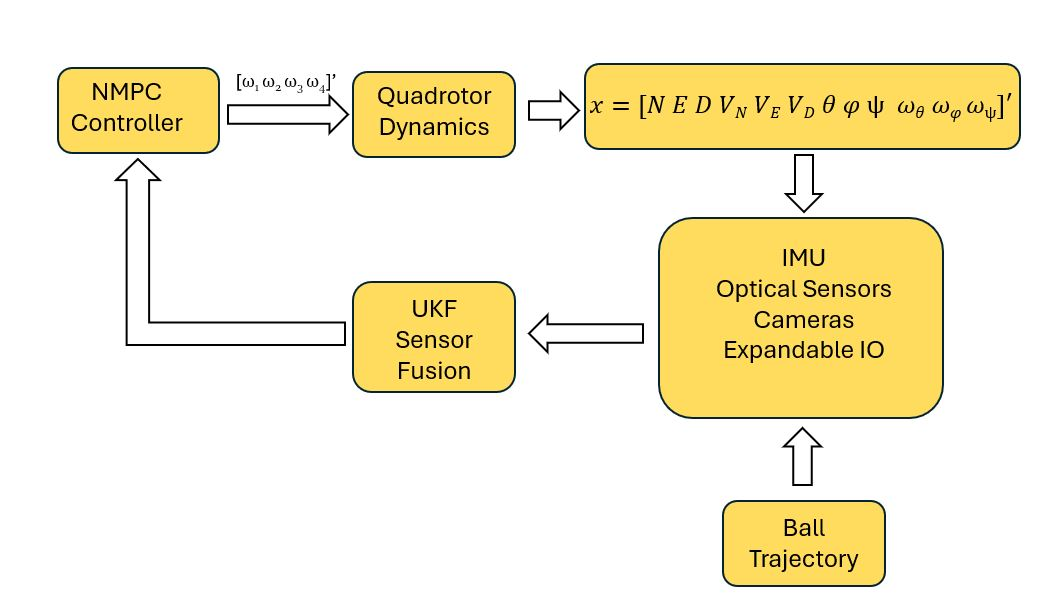
\includegraphics[width=\linewidth]{Figures/High Level Block Diagram.JPG}
    \caption{High-level block diagram of the quadrotor system for catching a ball.}
    \label{fig:HighLevelBlockDiagram} % Add label for referencing
\end{figure}
\section{Quadrotor Dynamics}
\subsection{Mathematical Model}
\subsubsection{Assumptions}
In developing the quadrotor dynamics for the NMPC control system, several key assumptions were made to simplify the model and focus on the primary control objectives:

\begin{itemize}
    \item The quadrotor is modelled as a rigid structure with no flexible parts.
    \item It is assumed to be symmetrical around both the pitch and roll axes.
    \item Thrust and forces are considered to be directly proportional to the propeller speed.
    \item Drag is neglected.
    \item The effects of blade flapping are neglected.
    \item Gravity is assumed to be constant, with variations due to height being negligible due to the indoor scenario.
    \item The presence of wind is not considered in the model.
    \item Ground effect is considered negligible and thus not included in the model.
\end{itemize}

These assumptions allow for a more tractable analysis and control design, focusing on the primary dynamics and control challenges of the quadrotor.

\subsubsection{Coordinates and Rotation Matrices}

For the Quanser quadrotor model, a North-East-Down (NED) coordinate system was used, where the north and east axes were defined between the rotors, considering sensor placement. In this system, the down direction is positive in the direction of gravity.-

To define the relationship between the body-fixed frame and the world frame, rotation matrices about the roll (\(\phi\)), pitch (\(\theta\)), and yaw (\(\psi\)) axes are used \cite{website:RotationMatricies}. These matrices are crucial for transforming vectors between frames.

The rotation matrices are:
\begin{equation}
    R_x(\phi) = \begin{bmatrix}
    1 & 0 & 0 \\
    0 & \cos\phi & -\sin\phi \\
    0 & \sin\phi & \cos\phi
    \end{bmatrix}
    \label{eq:rotation_matrix_x}
    \end{equation}
    
    \begin{equation}
    R_y(\theta) = \begin{bmatrix}
    \cos\theta & 0 & \sin\theta \\
    0 & 1 & 0 \\
    -\sin\theta & 0 & \cos\theta
    \end{bmatrix}
    \label{eq:rotation_matrix_y}
    \end{equation}
    
    \begin{equation}
    R_z(\psi) = \begin{bmatrix}
    \cos\psi & -\sin\psi & 0 \\
    \sin\psi & \cos\psi & 0 \\
    0 & 0 & 1
    \end{bmatrix}
    \label{eq:rotation_matrix_z}
    \end{equation}
    

The composite rotation matrix \(R\) is formed by multiplying these matrices:

\begin{equation}
    R = R_z(\psi) R_y(\theta) R_x(\phi)
    \label{eq:combined_rotation_matrix}
    \end{equation}
    
    \begin{equation}
    R = \begin{bmatrix}
    \cos\psi \cos\theta & \cos\psi \sin\theta \sin\phi - \sin\psi \cos\phi & \cos\psi \sin\theta \cos\phi + \sin\psi \sin\phi \\
    \sin\psi \cos\theta & \sin\psi \sin\theta \sin\phi + \cos\psi \cos\phi & \sin\psi \sin\theta \cos\phi - \cos\psi \sin\phi \\
    -\sin\theta & \cos\theta \sin\phi & \cos\theta \cos\phi
    \end{bmatrix}
    \label{eq:expanded_rotation_matrix}
    \end{equation}
    

This matrix \(R\) is essential for transforming coordinates between the world and body frames, playing a significant role in accurately simulating the quadrotor's behaviour and calculating forces and torques.

By using the NED coordinate system and these rotation matrices, the relationship between the world frame and the body frame is clearly established, enabling precise modelling and control of the Quanser quadrotor.

\subsubsection{States and Inputs}
To fully describe the condition of the system at any given time, a set of states must be assigned to encompass all the dynamic behaviour. For this system, the states are defined as:

\begin{itemize}
    \item \text{N}: Position in the north direction (world frame).
    \item \text{E}: Position in the east direction (world frame).
    \item \text{D}: Position in the down direction (world frame, positive in the direction of gravity).
    \item \text{\(\dot{N}\)}: Velocity in the north direction (world frame).
    \item \text{\(\dot{E}\)}: Velocity in the east direction (world frame).
    \item \text{\(\dot{D}\)}: Velocity in the down direction (world frame).
    \item \text{\(\phi\)}: Roll angle, describing rotation around the north axis (world frame).
    \item \text{\(\theta\)}: Pitch angle, describing rotation around the east axis (world frame).
    \item \text{\(\psi\)}: Yaw angle, describing rotation around the down axis (world frame).
    \item \text{\(\dot{\phi}\)}: Angular velocity around the north axis (world frame).
    \item \text{\(\dot{\theta}\)}: Angular velocity around the east axis (world frame).
    \item \text{\(\dot{\psi}\)}: Angular velocity around the down axis (world frame).
\end{itemize}

These states collectively capture the position, orientation, and motion dynamics of the system and can be grouped into subsets depending on their effects. Specifically, \(\mathbf{X_n} = [N, E, D]\) represents the position, \(\mathbf{W_n} = [\phi, \theta, \psi]\) represents the orientation, \(\mathbf{\dot{X}_n} = [\dot{N}, \dot{E}, \dot{D}]\) represents the linear velocities, and \(\mathbf{\dot{W}_n} = [\dot{\phi}, \dot{\theta}, \dot{\psi}]\) represents the angular velocities. Using all of these variables the states of the system are \(\mathbf{x} = [\mathbf{X_n}, \mathbf{\dot{X}_n}, \mathbf{W_n}, \mathbf{\dot{W}_n}]\)

Additionally, two crucial subgroups for system modelling are \(\mathbf{\dot{X}_B} = [u, v, w]\) and \(\mathbf{\dot{W}_B} = [p, q, r]\), the linear and angular velocities in the body coordinates. These are important because they allow for the transformation of velocities between the body and world frames as shown in Equations \ref{eq:velocity_transformation} and \ref{eq:angular_velocity_transformation} below \cite{HindawiDynamcis}:

\begin{equation}
\mathbf{\dot{X}_n} = R_{bn} \mathbf{\dot{X}_B}
\label{eq:velocity_transformation}
\end{equation}

\begin{equation}
\mathbf{\dot{W}_n} = W_n^{-1} \mathbf{\dot{W}_B}
\label{eq:angular_velocity_transformation}
\end{equation}
    

where \(R\) is the rotation matrix (\ref{eq:expanded_rotation_matrix}) and \(W_n\) is the transformation matrix found in Appendix A.

The inputs to the quadrotor system are the individual angular velocities of each motor \(\mathbf{u} = [w_1, w_2, w_3, w_4]\). These inputs directly affect the thrust and torques generated by the rotors, influencing the quadrotor's movement and orientation, and are the controllable elements of the system.

\subsection{Motor Equations}
The thrust generated by a quadrotor motor is the primary driving force of the system. The thrust for each motor can be calculated using Equation \ref{eq:thrust} \cite{HindawiDynamcis}:

\begin{equation}
T_i = k_t \cdot \omega_i^2
\label{eq:thrust}
\end{equation}

where \(T_i\) is the individual thrust produced by motor \(i\) (i is the ith motor for example motor four is i = 4) in the body frame, \(k_t\) is the thrust coefficient, and \(\omega_i\) is the angular velocity of motor \(i\). The thrust coefficient \(k_t\) depends on the shape of the propeller and was determined through system identification performed by Quanser for their specific motors. The thrust generated by each motor directly influences the quadrotor's ability to lift, manoeuvre, and stabilize.
\subsection{Translational Dynamics}
To derive the translational equations of motion, Newton's second law of motion, \( F = ma \), is utilized in global coordinates. This can be expressed as:

\begin{equation}
\sum \mathbf{F} = m \mathbf{\ddot{X}}
\label{eq:newton_law}
\end{equation}

In this equation, \(\sum \mathbf{F}\) represents the sum of all external forces acting on the system, \(m\) denotes the mass of the system, and \(\mathbf{\ddot{X}}\) is the linear acceleration of the system. By rearranging this equation we can solve for linear acceleration of the system.

The sum of forces on the system can be defined as:

\begin{equation}
\sum \mathbf{F} = \mathbf{F}_g - \mathbf{F}_T - \mathbf{F}_d
\label{eq:sum_of_forces}
\end{equation}

where \(\mathbf{F}_g\) is the force of gravity, \(\mathbf{F}_T\) is the total thrust, and \(\mathbf{F}_d\) is the drag force. As stated in the assumptions we neglect the force of drag in this analysis.

The gravitational force, \(\mathbf{F}_g\), is given by \(mg\), where \(m\) is the mass of the quadrotor and \(g\) is the acceleration due to gravity. In the coordinate system, this force can be represented as \([0 \ 0 \ mg]^T\) because it acts only in the \(D\)-direction.

Similarly, the total thrust, \(\mathbf{F}_T\), acts only in the \(D\)-direction. Therefore, it can be represented as \([0 \ 0 \ -F_T]^T\), where \(F_T\) is the magnitude of the total thrust generated by the quadrotor's motors. This can be seen in Equation \ref{eq:forceThrust}.


\begin{equation}
    \mathbf{F}_T = R \sum \mathbf{T}_i
    \label{eq:forceThrust}
    \end{equation}

Where \( R \) is the rotation matrix required to transform the force from body to earth coordinates and \( \mathbf{T}_i \) is the result of Equation \ref{eq:thrust}.
After deriving these expressions the linear acceleration of the quadrotor can be found \cite{website:Quadrotorsystemmodeling}.

\subsection{Rotational Dynamics}

\subsection{State Space Equations of Motion}

\section{NMPC}

Choosing Nonlinear Model Predictive Control (NMPC) for the drone project, where the objective is to catch a thrown ball, provides several critical advantages over other control methods. NMPC's ability to incorporate constraints directly into the control design is particularly valuable. By defining specific constraints on the drone's motor velocities and their rates of change, safe and efficient operation within the drone's physical limits can be ensured. The use of a prediction horizon in NMPC allows the controller to use the ball's estimated trajectory, provided by external systems like a Kalman filter, as a reference. This enables the drone to plan its movements proactively, enhancing the likelihood of a successful catch.

The control horizon enables fine-tuning of how far ahead the controller looks when making decisions, ensuring a balance between responsiveness and stability. This is crucial for quickly adapting to the ball's trajectory while maintaining controlled flight. The ability to precisely adjust the weighting of each state variable in NMPC is also essential, as it allows prioritization of certain aspects of the drone's behaviour, such as position accuracy and control effort.
\subsection{Implementation}

In implementing the NMPC for the drone within a simulation environment, specific values were carefully chosen for the controller's weights and constraints to optimize its performance for the task of catching a thrown ball. The controller is configured with a prediction horizon of 30 steps and a control horizon of 29 steps, ensuring a fast response to the dynamic task. The time step for the controller is set to 0.01 seconds, providing high-frequency updates for precise control.

The controller uses the following state weights to ensure precise control over the drone's position and orientation: [15, 15, 15, 1, 1, 1, 5, 5, 5, 1, 1, 1]. These weights emphasize the importance of accurate position tracking while also considering orientation and other dynamic aspects of the system. The manipulated variable weights are set to [0.5, 0.5, 0.5, 0.5], which help balance control effort and minimize excessive actuator use. Additionally, the rate of change weights for the manipulated variables are [0.2, 0.2, 0.2, 0.2], which further ensure smooth control actions and prevent abrupt changes that could destabilize the drone.

Constraints are also defined to keep the drone's operation within safe and efficient limits. The motor velocities are constrained to a minimum of 0 and a maximum of 20, with rate limits set between -5 and 5. These constraints ensure that the motors operate within their physical capabilities and provide a safe response to control commands.

Currently, the NMPC uses the default cost function, which balances state tracking and control effort. In future iterations, I plan to customize this cost function to better suit the specific requirements of intercepting a moving ball, potentially enhancing the controller's performance even further.

By carefully setting these parameters, the NMPC is tailored to provide robust and efficient control, enabling the drone to effectively track and intercept the ball's trajectory while maintaining stability and precision in the simulation environment.

\section{Simulation}
\subsection{Setup and Validation}

After establishing the dynamics, a simulation was created to validate the controller and system performance. This simulation initializes the drone's parameters and specifies the starting states. The main simulation loop uses the ODE45 solver \cite{website:KalmanFilter} to get state updates and the NMPC toolbox \cite{website:NMPCSIM} to drive the control variables. The first test to check the dynamics involved manually setting all inputs to 4.9, which balances out gravity and allows the drone to hover, confirming the dynamics were correctly modeled. Following this, a simple trajectory was set for the drone to follow. The drone successfully tracked the trajectory, verifying the controller's effectiveness.

The assessment of performance was done not only through graphical information but also visually through animation. By graphing the states and inputs and animating the drone's movement, the system's correct behavior and control responses were confirmed. This successful validation allowed the progression to simulating the drone catching a ball.

\subsection{Ball Trajectory and Assumptions}

For the simulation of the drone intercepting a thrown ball, the ball's trajectory is generated using a series of assumptions and random initial conditions. In a real-world scenario, a Vicon system would be used to obtain the ball's velocity, angle, and other necessary parameters. However, for the current simulation, these parameters are randomly generated to simulate different possible trajectories of the ball.
The initial conditions for the ball's trajectory can be visualized in Figure \ref{fig:Projectilemotion}, including a random initial velocity \(V_o\) and random initial angles in both vertical (\(\theta\)) and horizontal (\(\psi\)) directions. The ball is assumed to be thrown from a height of 1.5 meters. When the drone intercepts the ball is determined based on the height at which interception is desired, allowing control over the drone's height suitable for an indoor setting.



\newpage
\begin{figure}[H]
    \centering
    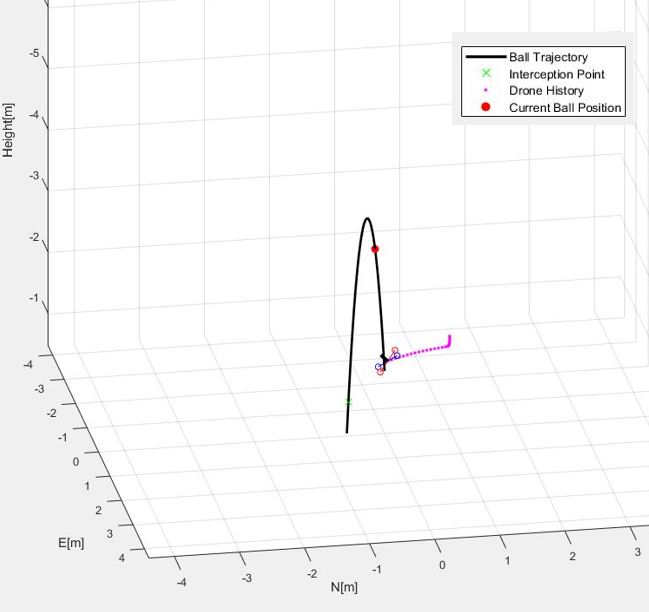
\includegraphics[width=1\linewidth]{Figures/animationwithlegend.JPG}
    \caption{Screenshot of the quadrotor animation.}
    \label{fig:Projectilemotion} % Add label for referencing
\end{figure}

Assuming perfect projectile motion for simplicity, the trajectory of the ball is calculated, and the time of flight is determined based on the initial conditions and the ball's physical properties. If the calculated time of flight is infeasible for the drone to intercept the ball (less than 1 second), the simulation stops, indicating that the scenario is unrealistic.

The initial velocity, angles, and resulting trajectory provide a reference for the NMPC controller, which is tasked with manoeuvring the drone to intercept the ball. This setup allows for the testing and validation of the drone's ability to follow and intercept the ball's path accurately.

The ball's trajectory is visualized along with the drone's movement in the simulation, allowing for both graphical analysis, as shown in Figure \ref{fig:simResults}, and animation of the interception process. This dual approach ensures that the system's behaviour can be thoroughly assessed, providing insights into the performance of the controller and the dynamics of the drone in various interception scenarios.


\subsection{Results}
The simulation effectively allows for tuning and testing of the NMPC controller designed for the drone to intercept a thrown ball. Initial results indicate that while the controller is operational, there is a need for further fine-tuning to improve performance.

Examining the simulation results, it is evident that the controller is currently experiencing issues with overshooting and fine position control on the interception point. This behaviour suggests that the drone might be heading directly to the predicted interception point rather than adjusting its trajectory to catch the ball more effectively.

\begin{figure}[H]
    \centering
    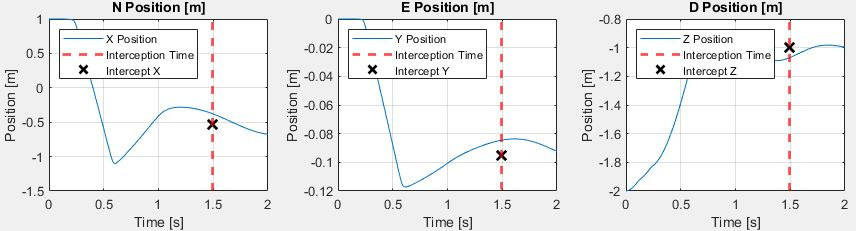
\includegraphics[width=1\linewidth]{Figures/SimResults.JPG}
    \caption{Quadrotor N E and D positions compared to the intercept location and time.}
    \label{fig:simResults} % Add label for referencing
\end{figure}

Overall however, the simulation is a success and will be a valuable tool as the project 

\section{Considerations Moving Forward}

Moving forward, the focus will be on enhancing the drone's capability to capture the ball with a more sophisticated strategy. Instead of simply intercepting the ball at a point in space, the goal is for the drone to anticipate the ball's trajectory and position itself at a point on the trajectory before the ball arrives. This approach will enable the drone to move down and perform a more controlled catch rather than a mere interception. Achieving this requires the drone to have a better understanding of the ball's location and its future path.

To attain the fine control necessary for this advanced manoeuvre, it may be essential to implement a custom cost function within the NMPC framework. This custom cost function will allow for more precise tuning of the controller, emphasizing the importance of positioning and timing in the catching process. Additionally, extensive tuning of the controller's parameters will be required to ensure optimal performance.

Once the drone is capable of gently and accurately catching the ball, the next step will be to integrate an obstacle avoidance feature. This feature will involve generating a trajectory that takes the drone away from the ball instead of towards it, thereby avoiding the ball. This requires the drone to not only track the ball's position but also dynamically adjust its path to avoid a potential collision. Successfully integrating this capability will make the system more versatile and adaptable to different scenarios.

After achieving these milestones, the plan is to utilize the Vicon system for tracking both the ball and the drone in real-time. The Vicon system will provide precise and accurate position data, which will be crucial for improving the performance of the NMPC controller. The final implementation will involve integrating the simulation controller with ROS (Robot Operating System) to facilitate real-world testing and deployment.

These advancements will significantly enhance the drone's capabilities, making it more efficient and reliable in performing complex tasks such as catching a ball and avoiding it when necessary.

\newpage
%%%%%%%%%%%%%%%%%%%%%%%%%%%%%%%%
\bibliographystyle{ieeetr}
\bibliography{main} % This is the .bib file where the bibliography database is stored
\appendix
\newpage


\end{document}
